\section[Boosting and AdaBoost]{Boosting and AdaBoost}

\subsection[Introduction]{Introduction}

\begin{frame}{Motivation for Boosting}
	\begin{itemize}
		\item We have seen that Random Forests manage the bias-variance trade-off by using an \textbf{ensemble} of models.
		\item The core idea was to train multiple trees with aggressive settings (high variance) in parallel (on bootstrapped training data), allowing the ensemble to reduce variance by averaging the predictions.
		\item \textbf{Boosting} approaches the problem differently: multiple trees with highly conservative settings (high bias) are trained \textbf{sequentially} on the training data, and a final weighted vote corrects the model's bias.
	\end{itemize}
\end{frame}

\begin{frame}{General Idea of Boosting}
	The core principle of Boosting can be summarized in the following points:
	\begin{itemize}
		\item We choose a conservative configuration for a base tree (typically limiting its maximum depth between 1 and 4). This tree exhibits high bias. We also set the total number of trees to train in the ensemble.
		\pause
		\item We train the first tree on the training data and evaluate its errors. This will later determine the voting importance that this tree holds during decision-making.
		\pause
		\item We assign a higher weight to the observations misclassified by this tree, which subsequently forms the updated training dataset.
		\pause
		\item We train a second tree by repeating the identical steps described above for the first tree.
		\pause
		\item And so on until all the trees in the sequence have been fully trained.
		\pause
		\item Boosting belongs to the family of \textbf{ensemble methods} in machine learning.
	\end{itemize}
\end{frame}

\begin{frame}{Weak Learners}
	In the AdaBoost (Adaptive Boosting) algorithm, the underlying base models must be very simple. They are formally referred to as \textbf{weak learners}.
	\begin{itemize}
		\item In practice, a decision tree of depth 1 is most frequently used, known as a \textbf{decision stump}.
		\pause
		\item A decision stump performs exactly one split on a single feature.
		\pause
		\item The depth can be slightly increased (e.g., 2 to 4) to allow the model to capture \textbf{interactions} between multiple variables (e.g., crossed pixels in an image).
		\pause
		\item The objective is not for each individual tree to be perfect. The global performance stems entirely from the \textbf{sequence}.
	\end{itemize}
\end{frame}

\subsection[Algorithm]{Algorithm}

\begin{frame}{The CART Algorithm with Weights}
	For Boosting to function properly, our decision tree must be capable of paying more attention to certain observations than others. We introduce a weight $w_i$ for each observation $i$.
	
	\vspace{0.3cm}
	The entropy formula remains unchanged. However, the proportion (probability) of a given class $k$ within a node is no longer based on individual counts, but on the \textbf{sum of their weights}.
	
	\pause
	\vspace{0.3cm}
	
	In a given group, the probability of obtaining class $k$ is calculated as:
	\begin{equation*}
		P(Y = k) = \frac{\sum_{i \in \text{group} \mid y^{(i)} = k} w^{(i)}}{\sum_{i \in \text{group}} w^{(i)}}
	\end{equation*}
	
	\pause
	
	This formula serves two crucial purposes:
	\begin{itemize}
		\item \textbf{For splitting:} It enables the calculation of the node's weighted entropy.
		\item \textbf{For prediction:} If the node is a leaf, the class predicted by the tree is the one with the highest weighted probability.
	\end{itemize}
\end{frame}

\begin{frame}{Weighted Calculation Example}
	Suppose we have a group containing the following observations:
	\begin{table}
		\centering
		\begin{tabular}{|l|c|c|c|c|}
			\hline
			\textbf{Observation} $i$ & 1 & 2 & 3 & 4 \\
			\hline
			\textbf{Class} $y^{(i)}$ & 0 & 1 & 0 & 1 \\
			\hline
			\textbf{Weight} $w^{(i)}$ & 0.33 & 0.20 & 0.27 & 0.20 \\
			\hline
		\end{tabular}
	\end{table}
	We compute the following probabilities:
	\begin{equation*}
		\begin{cases}
			P(Y = 0) = \frac{0.33 + 0.27}{1} = 0.6 \\
			P(Y = 1) = \frac{0.20 + 0.20}{1} = 0.4
		\end{cases}
	\end{equation*}
	The entropy $H(Y)$ is calculated as follows:
	\begin{equation*}
		\begin{aligned}
			H(Y) 
			&= \sum_{k=0}^1 P(Y = k) I(Y = k) \\
			&= - P(Y = 0) \log P(Y = 0) - P(Y = 1) \log P(Y = 1) \\
			&= - 0.6 \log 0.6 - 0.4 \log 0.4 \\
			&\approx 0.673
		\end{aligned}
	\end{equation*}
\end{frame}

\begin{frame}{Initialization and Error}
	For a $K$-class classification problem, we will use the multi-class generalization of AdaBoost known as \textbf{SAMME}:
	\begin{enumerate}
		\item We initialize all observations with equal weights: $w_1^{(i)} = \frac{1}{n}$.
		\pause
		\item For each tree $m$ from $1$ to $M$, we train tree $m$ on the weighted data. We then compute its \textbf{weighted error} $\epsilon_m \in [0, 1]$, which is the sum of the weights of the misclassified observations:
		\begin{equation*}
			\epsilon_m = \frac{\sum_{i=1}^n w_m^{(i)} \mathds{1}(\hat{f}_m(x^{(i)}) \neq y^{(i)})}{\sum_{i=1}^n w_m^{(i)}}
		\end{equation*}
		Where $\hat{f}_m(x^{(i)})$ is the prediction of tree $m$ for observation $i$, and $\mathds{1}$ is the indicator function (which equals $1$ if the condition is true and $0$ otherwise).
		\pause
		\item We check a early-stopping criterion: if $\epsilon_m \ge (K - 1)/ K$, boosting stops prematurely (resulting in fewer than $M$ trees). This occurs because the tree performs worse than random guessing.
	\end{enumerate}
\end{frame}

\begin{frame}{Computing the Tree's Voting Weight}
	Once the error $\epsilon_m$ is obtained, we determine the importance or \textbf{voting weight} of tree $m$, denoted by $\alpha_m \in \R^+$. The more accurate the tree, the larger its weight:
	
	\begin{equation*}
		\alpha_m = \nu \left[\log \left( \frac{1 - \epsilon_m}{\epsilon_m + \delta} \right) + \log(K - 1)\right]
	\end{equation*}
	
	\pause
	\vspace{0.3cm}
	The term $\log(K - 1)$ guarantees that the tree's weight remains positive as long as its error $\epsilon_m$ is strictly less than $(K-1)/K$. The parameter $\delta$ is a tiny numerical constant added to avoid division by zero (typically $10^{-8}$). Finally, $\nu$ represents the \textbf{learning rate}. It modulates the magnitude of the observation weight adjustments (see below). A typical value is $\nu = 1$; a smaller value will require a larger number of trees. It is therefore a key hyperparameter of AdaBoost.
\end{frame}

\begin{frame}{Voting Weight Calculation Example}
	In our MNIST classification problem, we have $K = 10$:
	\begin{itemize}
		\item A baseline classifier making purely random guesses has a 10\% chance of providing a correct answer, and consequently has a 90% chance of making an error. Therefore, if $\epsilon_m \ge 0.9$, the tree performs worse than random guessing, triggering an early stop.
		\item An algorithm exhibiting an error rate of $\epsilon_m = 0.89$ is poor but still marginally better than random guessing. Assuming $\nu = 1$:
		\begin{equation*}
			\begin{aligned}
				\alpha_m 
				&= \log \left( \frac{1 - \epsilon_m}{\epsilon_m + \delta} \right) + \log(K - 1) \\
				&= \log \frac{1 - 0.89}{0.89} + \log(10 - 1) \\
				&\approx 0.106
			\end{aligned}
		\end{equation*}
		The term $\log(K - 1)$ ensures a positive voting weight whenever the weak learner outperforms random guessing.
	\end{itemize}
\end{frame}

\begin{frame}{Updating Observation Weights}
	This is where the adaptive nature of the algorithm takes place (Adaptive Boosting). We update the weight of each observation $i$ for the transition to the subsequent tree $m+1$:
	
	\begin{equation*}
		w_{m+1}^{(i)} = w_m^{(i)} \exp\left(\alpha_m \mathds{1}(\hat{f}_m(x^{(i)}) \neq y^{(i)})\right)
	\end{equation*}
	
	\pause
	\begin{itemize}
		\item If the tree predicted correctly: $\mathds{1}(\hat{f}_m(x^{(i)}) \neq y^{(i)}) = 0$, meaning $\exp(0) = 1$. The weight \textbf{remains unchanged}.
		\item If the tree made an error: $\mathds{1}(\hat{f}_m(x^{(i)}) \neq y^{(i)}) = 1$. The weight is multiplied by $\exp(\alpha_m)$. It therefore \textbf{increases} more sharply when the tree achieved a low overall error rate $\epsilon_m$!
	\end{itemize}
	
	\vspace{0.3cm}
	Finally, we \textbf{normalize} all updated weights $w_{m+1}^{(i)}$ so that their sum equals $1$ once again before training the next tree in the sequence.
\end{frame}

\begin{frame}{Final Decision Making (The Vote)}
	Once all $M$ trees have been sequentially trained, the ensemble organizes a weighted vote to predict the class of a new observation $x$.
	
	\vspace{0.5cm}
	We accumulate the voting weights $\alpha_m$ of the trees that voted for each class $k$. For a given inference data point $x_i$, the winning class $\hat{f}(x_i)$ is the one that achieves the highest cumulative score:	
	\begin{equation*}
		\hat{f}(x_i) = \argmax{k} \sum_{m=1}^M \alpha_m \mathds{1}(\hat{f}_m(x_i) = k)
	\end{equation*}
\end{frame}

\begin{frame}{Probability Computation}
	Certain performance metrics (such as the Area Under the ROC Curve) require the model to output soft \textbf{probabilities} rather than hard class labels.
	
	\vspace{0.5cm}
	In AdaBoost, the probability of a class $k$ is obtained simply by calculating the \textbf{percentage of the total votes} (the voting weights) harvested by that class relative to the sum of the voting weights across all trees:
	
	\begin{equation*}
		P(Y = k \mid x_i) = \frac{\sum_{m=1}^M \alpha_m \mathds{1}(\hat{f}_m(x_i) = k)}{\sum_{m=1}^M \alpha_m}
	\end{equation*}
	
\end{frame}

\subsection[Case Study]{Case Study}

\begin{frame}{Simplification and Algorithms}
	We will train an AdaBoost model combined with a decision tree base estimator on the MNIST dataset, using a simplified version of the features obtained via Principal Component Analysis.
	
	\vspace{0.5cm}
	
	The Scikit-Learn algorithms we will utilize:
	\begin{itemize}
		\item \href{https://scikit-learn.org/stable/modules/generated/sklearn.decomposition.PCA.html}{\texttt{sklearn.decomposition.PCA}}
		\item \href{https://scikit-learn.org/stable/modules/generated/sklearn.tree.DecisionTreeClassifier.html}{\texttt{sklearn.tree.DecisionTreeClassifier}}
		\item \href{https://scikit-learn.org/stable/modules/generated/sklearn.ensemble.AdaBoostClassifier.html}{\texttt{sklearn.ensemble.AdaBoostClassifier}}
	\end{itemize}
\end{frame}

\begin{frame}{Example Results}
	Here is an example result obtained on the MNIST dataset using AdaBoost combined with a decision tree base estimator:
	\begin{columns}
		\begin{column}{0.5\textwidth}
			\begin{figure}
				\centering
				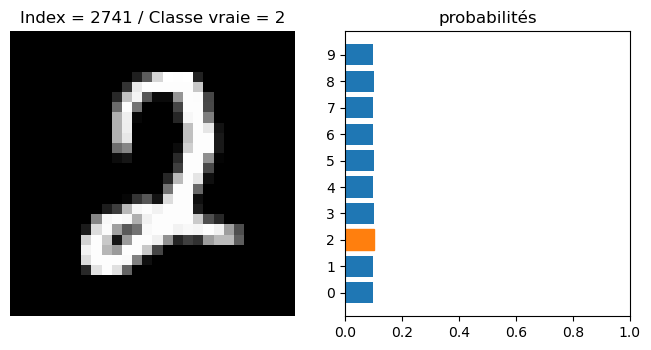
\includegraphics[width=1.0\linewidth]{Images/MNIST_3}
				\label{fig:MNIST_3}
			\end{figure}			
		\end{column}
		\begin{column}{0.5\textwidth}
			\begin{figure}
				\centering
				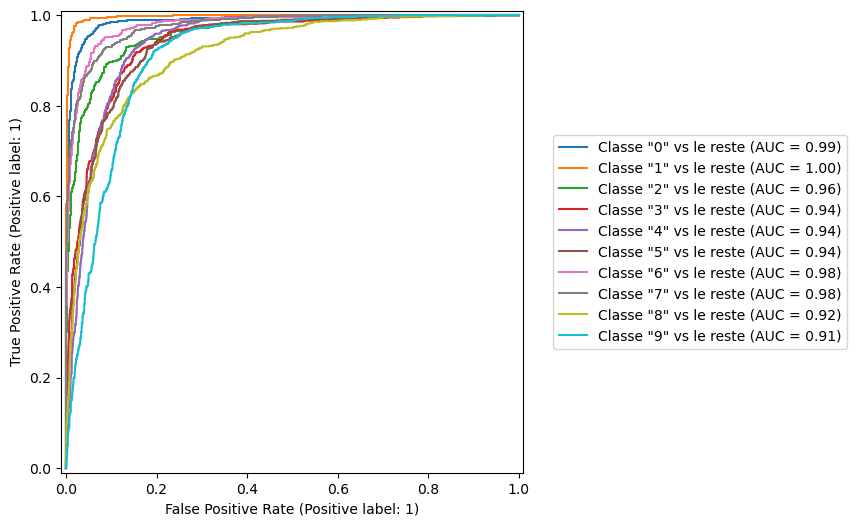
\includegraphics[width=1.0\linewidth]{Images/MNIST_4}
				\label{fig:MNIST_4}
			\end{figure}			
		\end{column}
	\end{columns}
	Note that AdaBoost does not actively seek to maximize the calculated probability for the true class, but merely to make it marginally larger than for the other classes. Simply looking at the ROC curves does not reveal this underlying behavior.
\end{frame}

\subsection[Summary]{Summary}

\begin{frame}{AdaBoost (SAMME)}
	\begin{figure}
		\centering
		\resizebox{\textwidth}{!}{
			\begin{tikzpicture}[
				>=stealth,
				node distance=1.2cm and 1.5cm,
				data/.style={circle, draw=black, fill=blue!10, minimum size=1.8cm, align=center, font=\footnotesize},
				tree/.style={rectangle, draw=black, fill=red!15, minimum width=2cm, minimum height=1cm, align=center, font=\footnotesize},
				agg/.style={rectangle, rounded corners, draw=black, fill=yellow!20, minimum width=4cm, minimum height=1cm, align=center},
				arrow/.style={thick, ->}
				]
				
				% Data nodes
				\node[data] (D1) {$\mathcal{D}$\\$w_1^{(i)}$ equal};
				\node[data, fill=purple!20] (D2) [right=2cm of D1] {$\mathcal{D}$\\$w_2^{(i)}$ updated};
				\node (Dots) [right=1.2cm of D2] {\Large \dots};
				\node[data, fill=red!30] (DM) [right=1.2cm of Dots] {$\mathcal{D}$\\$w_M^{(i)}$ updated};
				
				% Tree nodes
				\node[tree] (T1) [below=0.4cm of D1] {Tree 1\\(Stump)};
				\node[tree] (T2) [below=0.4cm of D2] {Tree 2\\(Stump)};
				\node[tree] (TM) [below=0.4cm of DM] {Tree $M$\\(Stump)};
				
				% Alpha weights
				\node[font=\footnotesize\color{red!70!black}] (A1) [below=0.05cm of T1, xshift=-0.8cm] {Weight: $\alpha_1$};
				\node[font=\footnotesize\color{red!70!black}] (A2) [below=0.05cm of T2, xshift=-0.8cm] {Weight: $\alpha_2$};
				\node[font=\footnotesize\color{red!70!black}] (AM) [below=0.05cm of TM, xshift=-0.8cm] {Weight: $\alpha_M$};
				
				% Vote Node
				\node[agg] (Vote) [below=2.0cm of D2] {Weighted Vote\\$\hat{f}(x_i) = \argmax{k} \sum_{m=1}^M \alpha_m \mathds{1}(\hat{f}_m(x_i) = k)$};
				\node (Out) [below=0.4cm of Vote] {\textbf{Prediction}};
				
				% Horizontal arrows (updates)
				\draw[arrow] (D1) -- (T1);
				\draw[arrow] (T1.east) -- node[above, sloped, font=\scriptsize] {Error $\epsilon_1$} node[below, sloped, font=\scriptsize] {Update $w_2^{(i)}$} (D2.south west);
				\draw[arrow] (D2) -- (T2);
				\draw[arrow] (T2.east) -- node[above, sloped, font=\scriptsize] {Error $\epsilon_2$} (Dots.south west);
				\draw[arrow] (DM) -- (TM);
				
				% Arrows to vote
				\draw[arrow, dashed] (T1.south) |- (Vote.west);
				\draw[arrow, dashed] (T2.south) -- (Vote.north);
				\draw[arrow, dashed] (TM.south) |- (Vote.east);
				
				\draw[arrow] (Vote) -- (Out);
				
			\end{tikzpicture}
		}
	\end{figure}
	\vspace{0.5cm}
	\textbf{Sequential} architecture. We reduce \textbf{bias} by chaining simple models together.
\end{frame}